% !TEX root = ../main.tex
%---------------------------------------------------------------------------------------------------
\subsection{Results}\label{Appendix results}\FloatBarrier
%---------------------------------------------------------------------------------------------------
Figure \ref{Model fit appendix} shows further comparisons between the simulated and empirical data. All results from the estimated model are based on $10,000$ individuals.

\begin{figure}[h]\centering
	\subfloat[White-collar]{\scalebox{0.25}{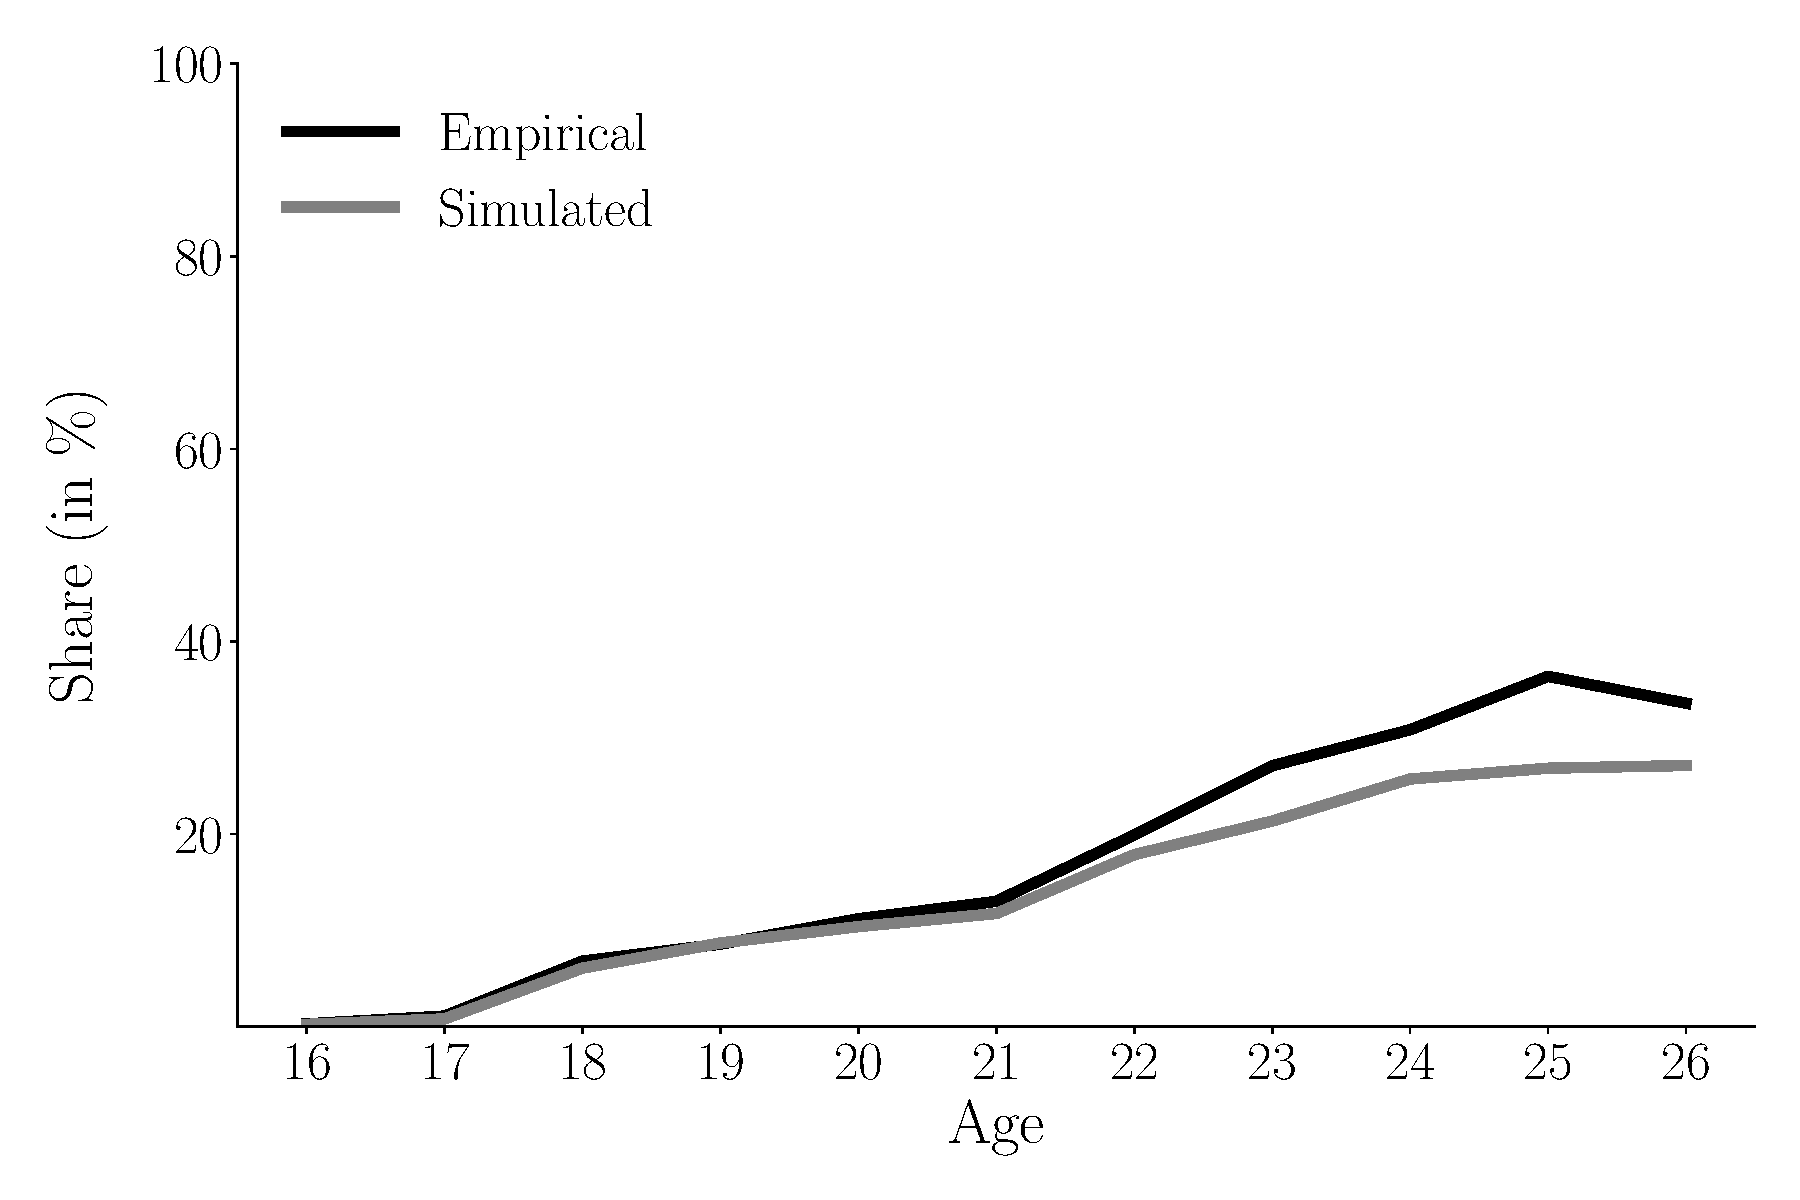
\includegraphics{fig-model-fit-choice-white-bw}}}
	\subfloat[Military]{\scalebox{0.25}{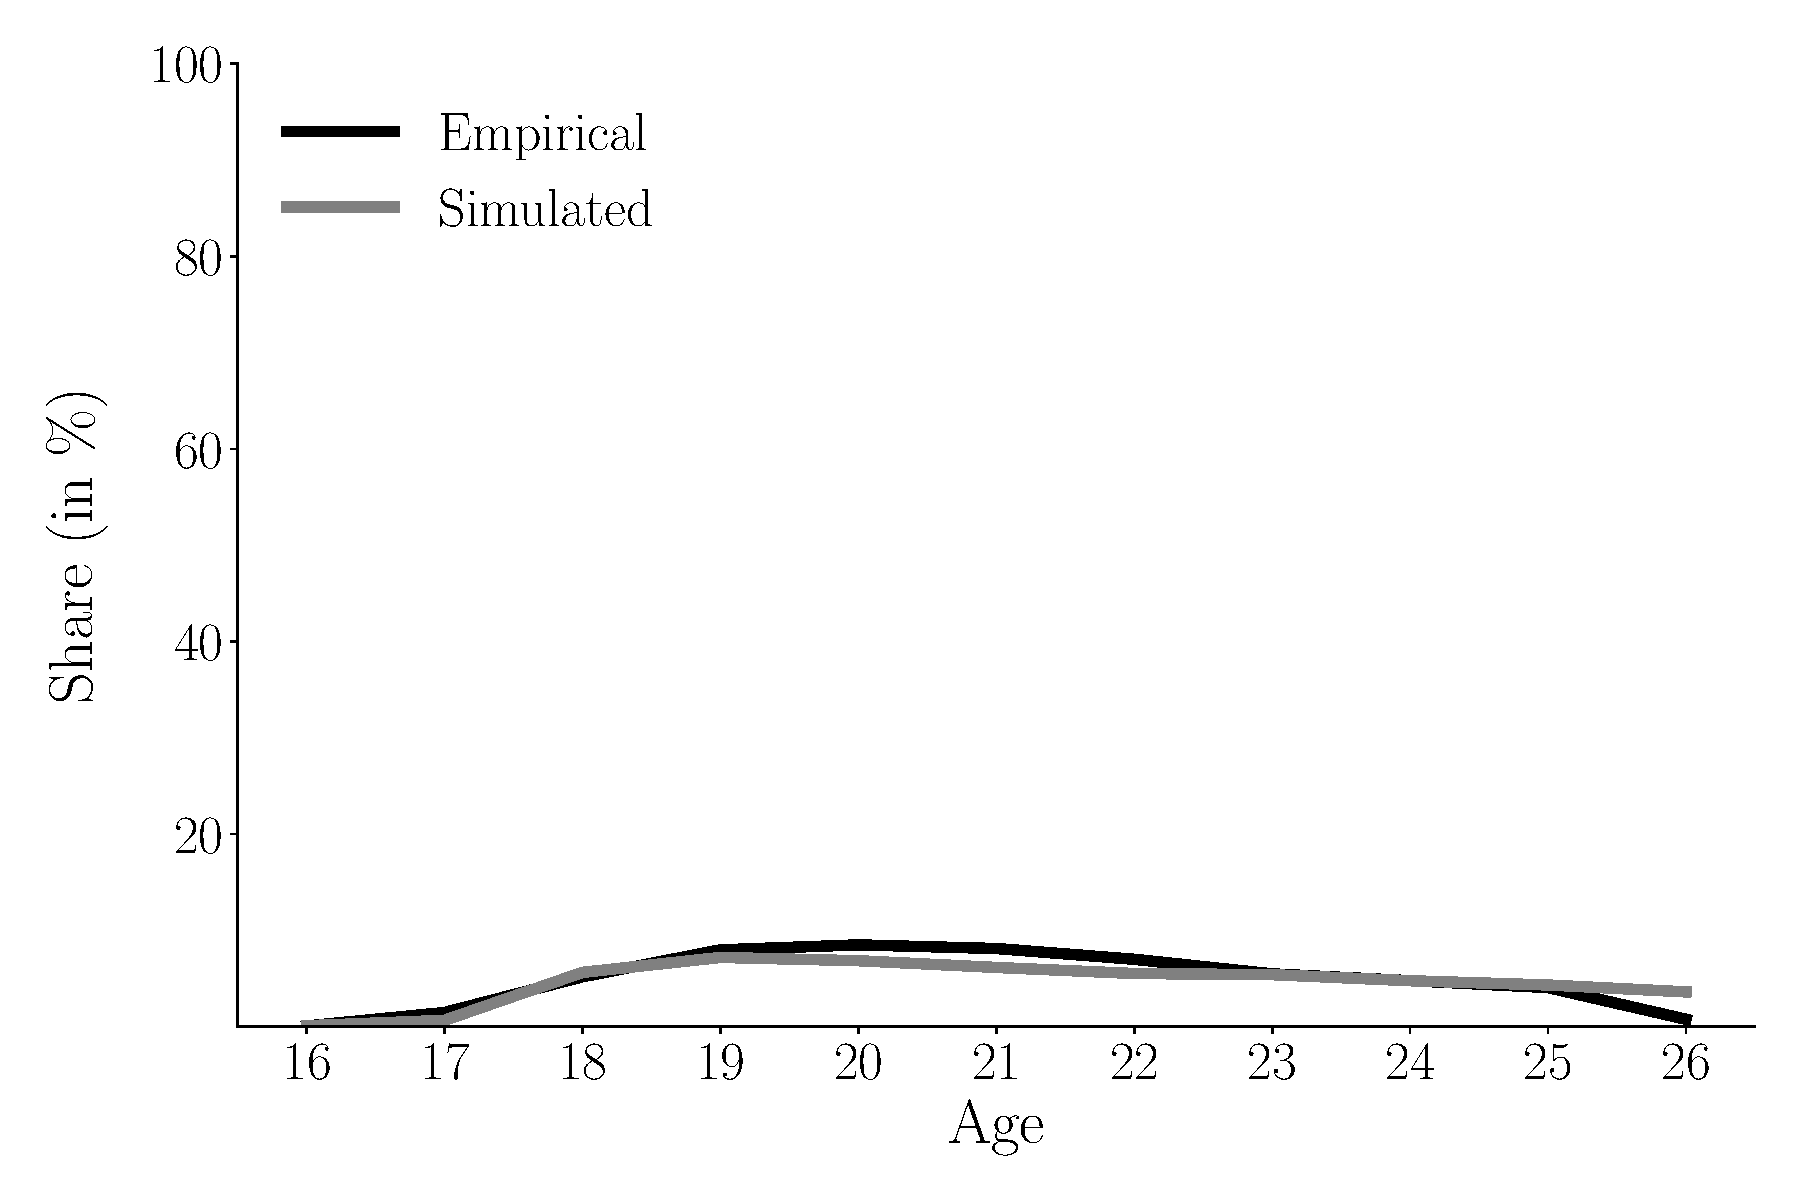
\includegraphics{fig-model-fit-choice-military-bw}}} \\
	\subfloat[School]{\scalebox{0.25}{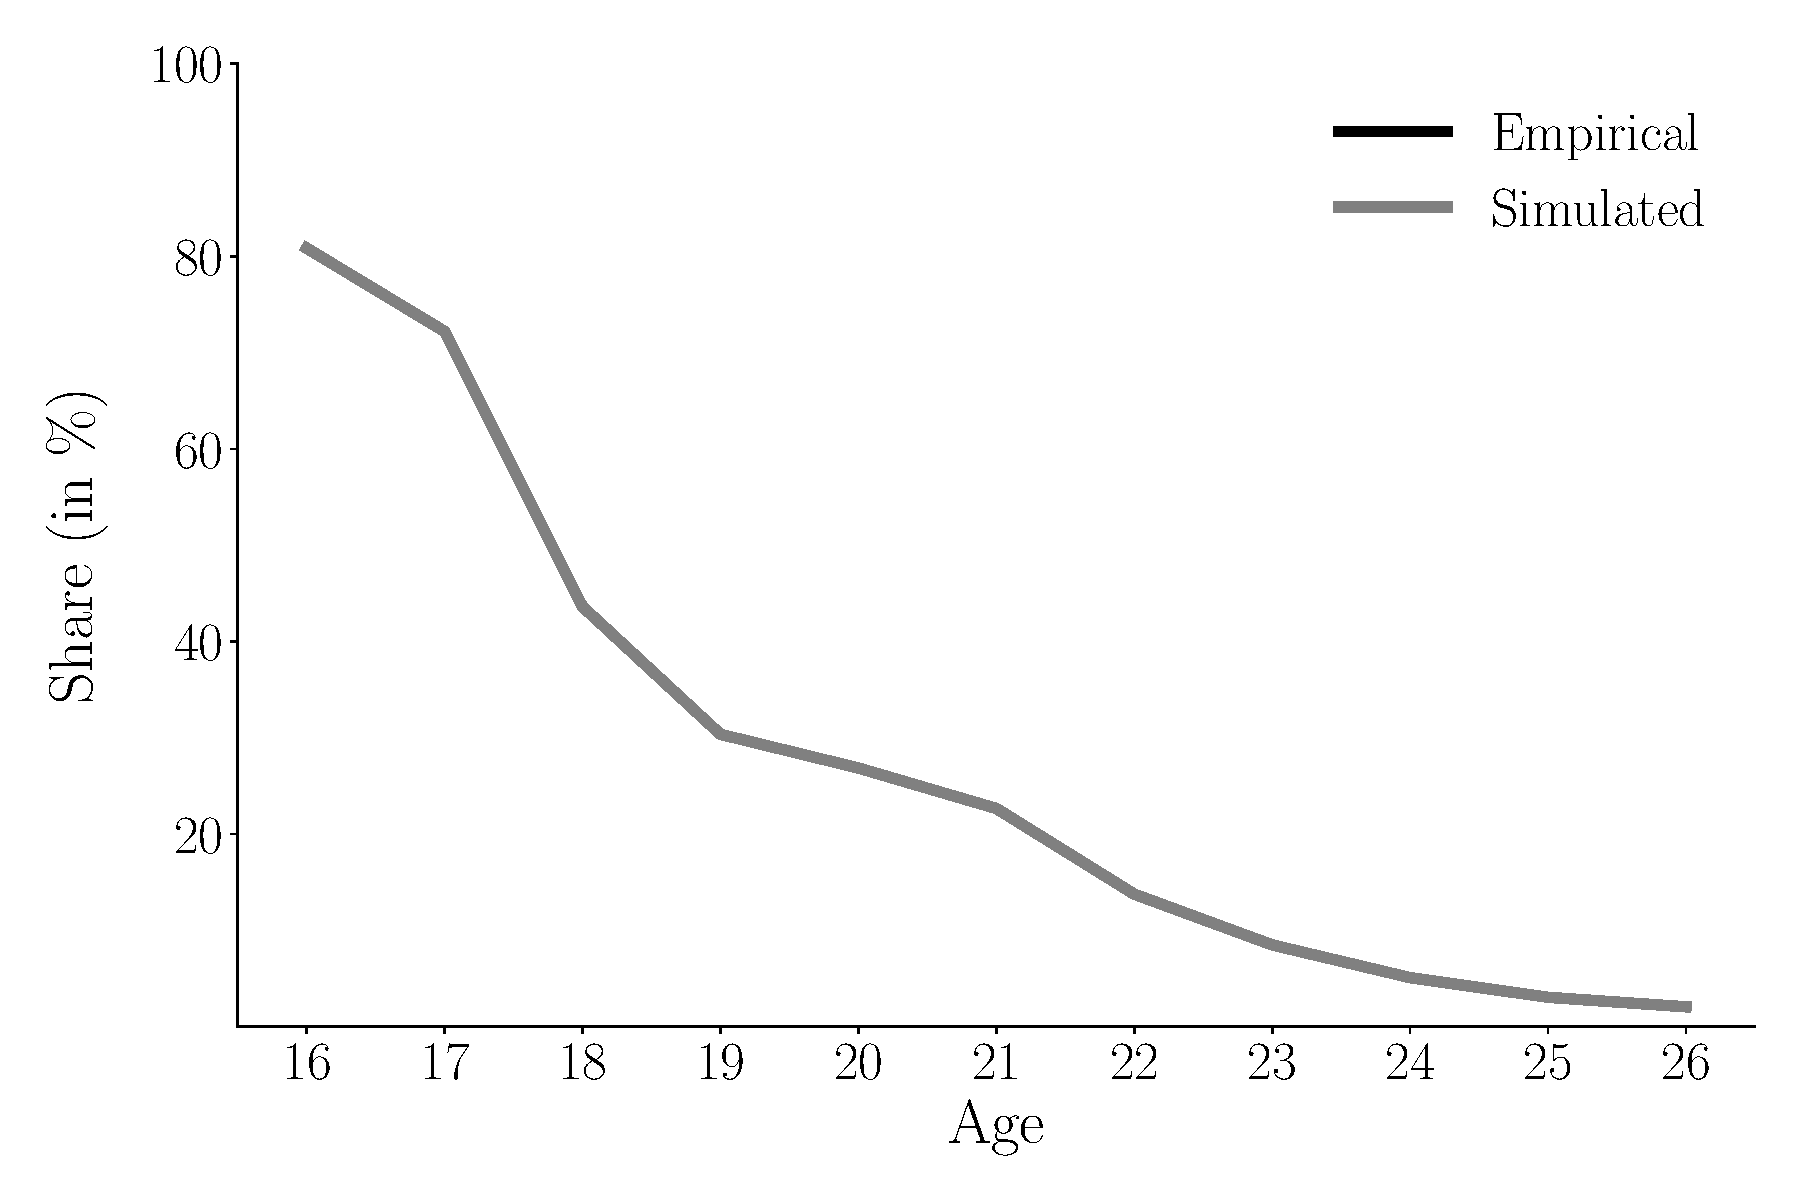
\includegraphics{fig-model-fit-choice-school-bw}}}
	\subfloat[Home]{\scalebox{0.25}{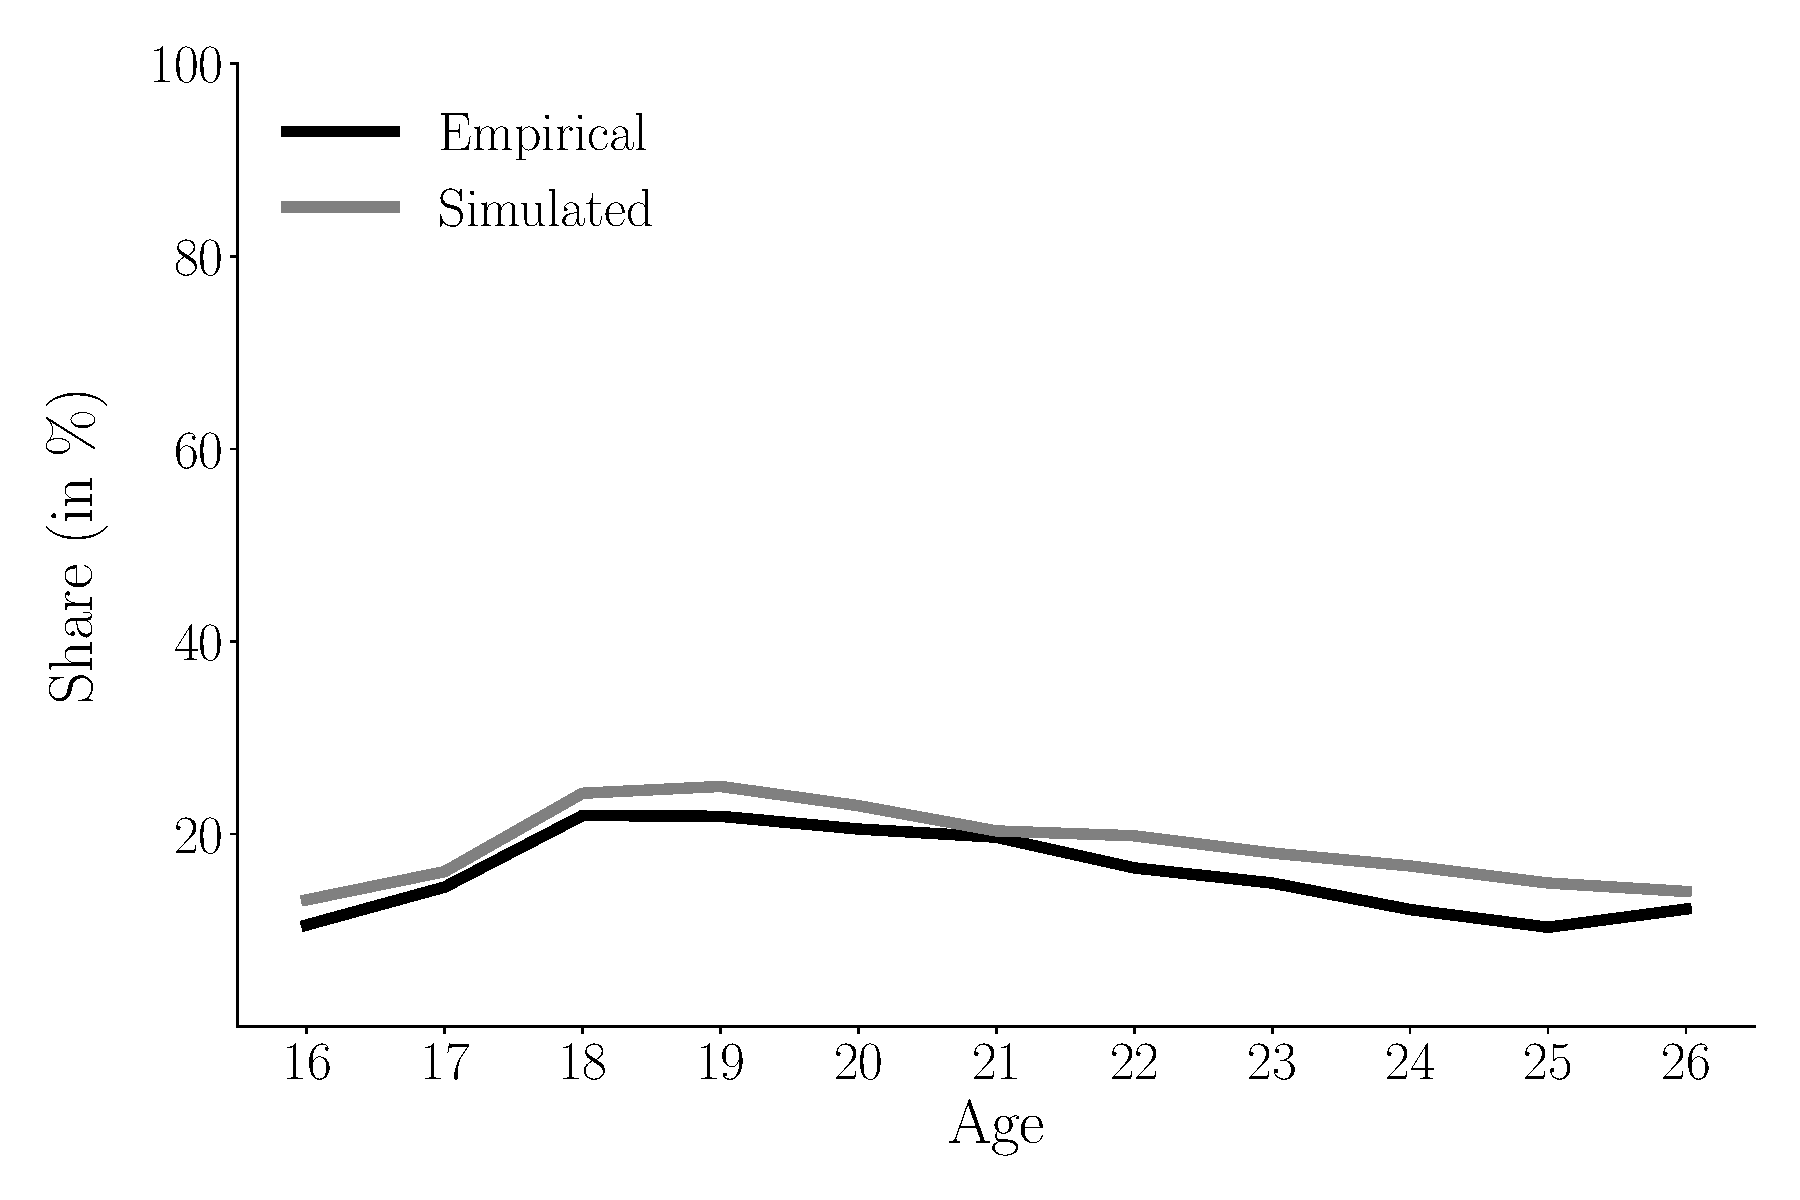
\includegraphics{fig-model-fit-choice-home-bw}}}
	\caption{Model fit}\label{Model fit appendix}
\end{figure}\FloatBarrier

\noindent Figure \ref{Targeted subsidy for all types} provides the point prediction, its sampling distribution, and the estimated confidence set for the impact of the tuition subsidy on all types. All results are based on $30,000$ draws from the asymptotic normal distribution of our parameter estimates.

\begin{figure}[h!]\centering
  \subfloat[Type 1]{\scalebox{0.25}{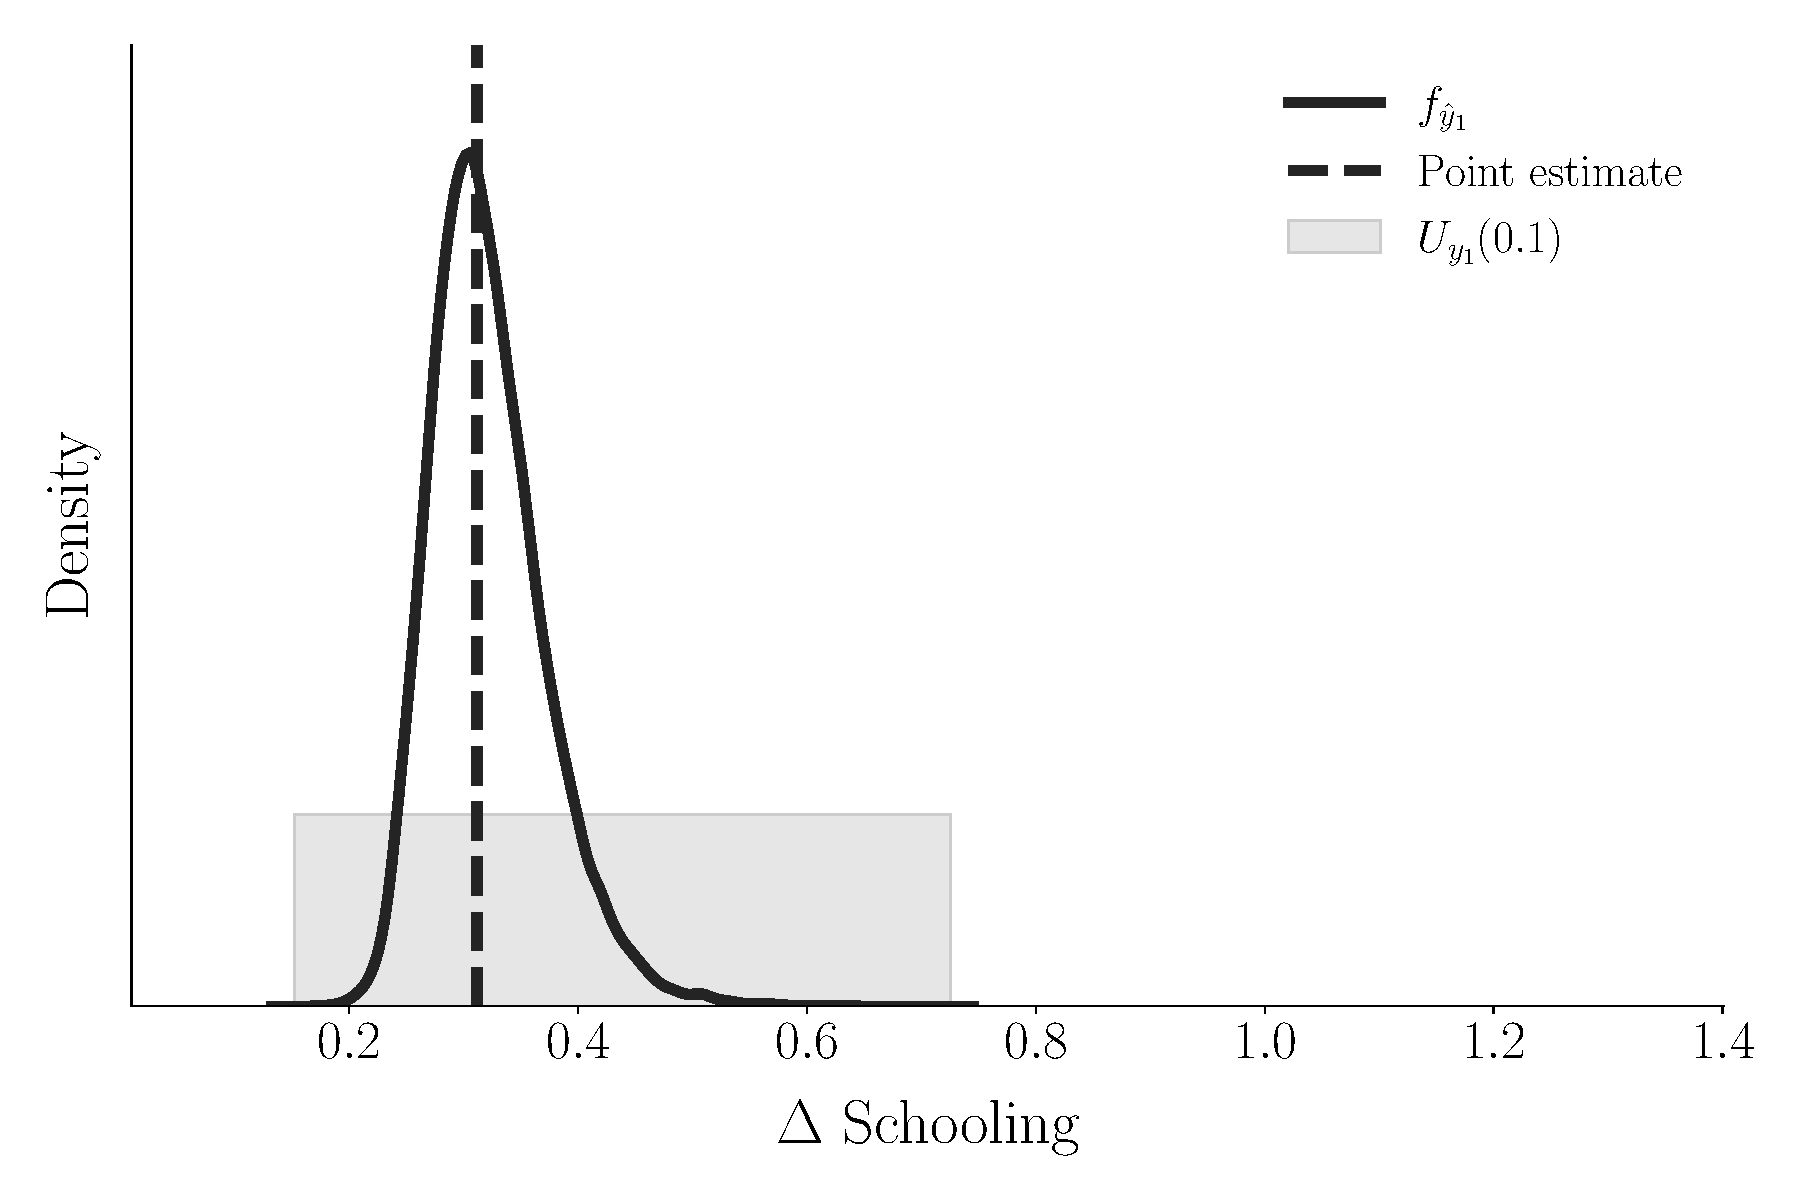
\includegraphics{fig-policy-average-years-type-0-bw}}}
  \subfloat[Type 2]{\scalebox{0.25}{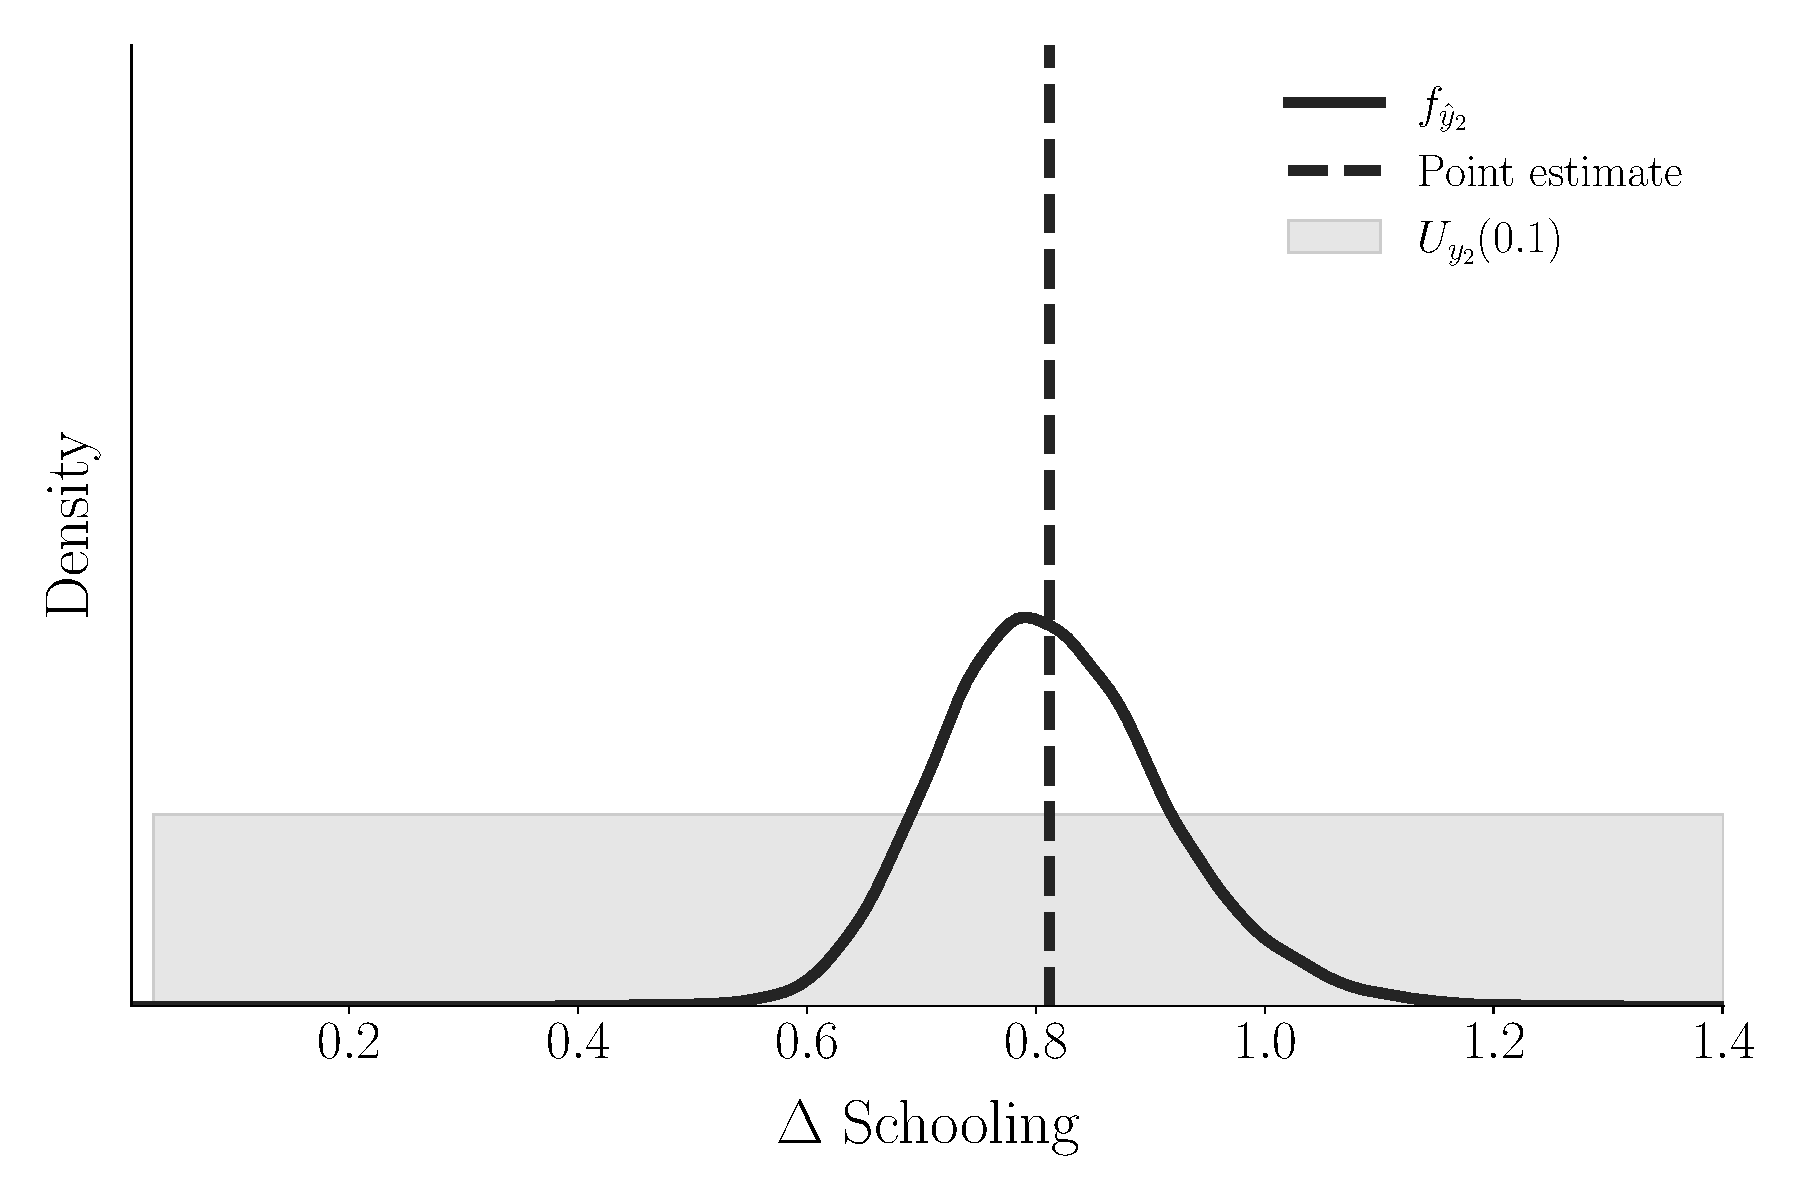
\includegraphics{fig-policy-average-years-type-1-bw}}}\\
  \subfloat[Type 3]{\scalebox{0.25}{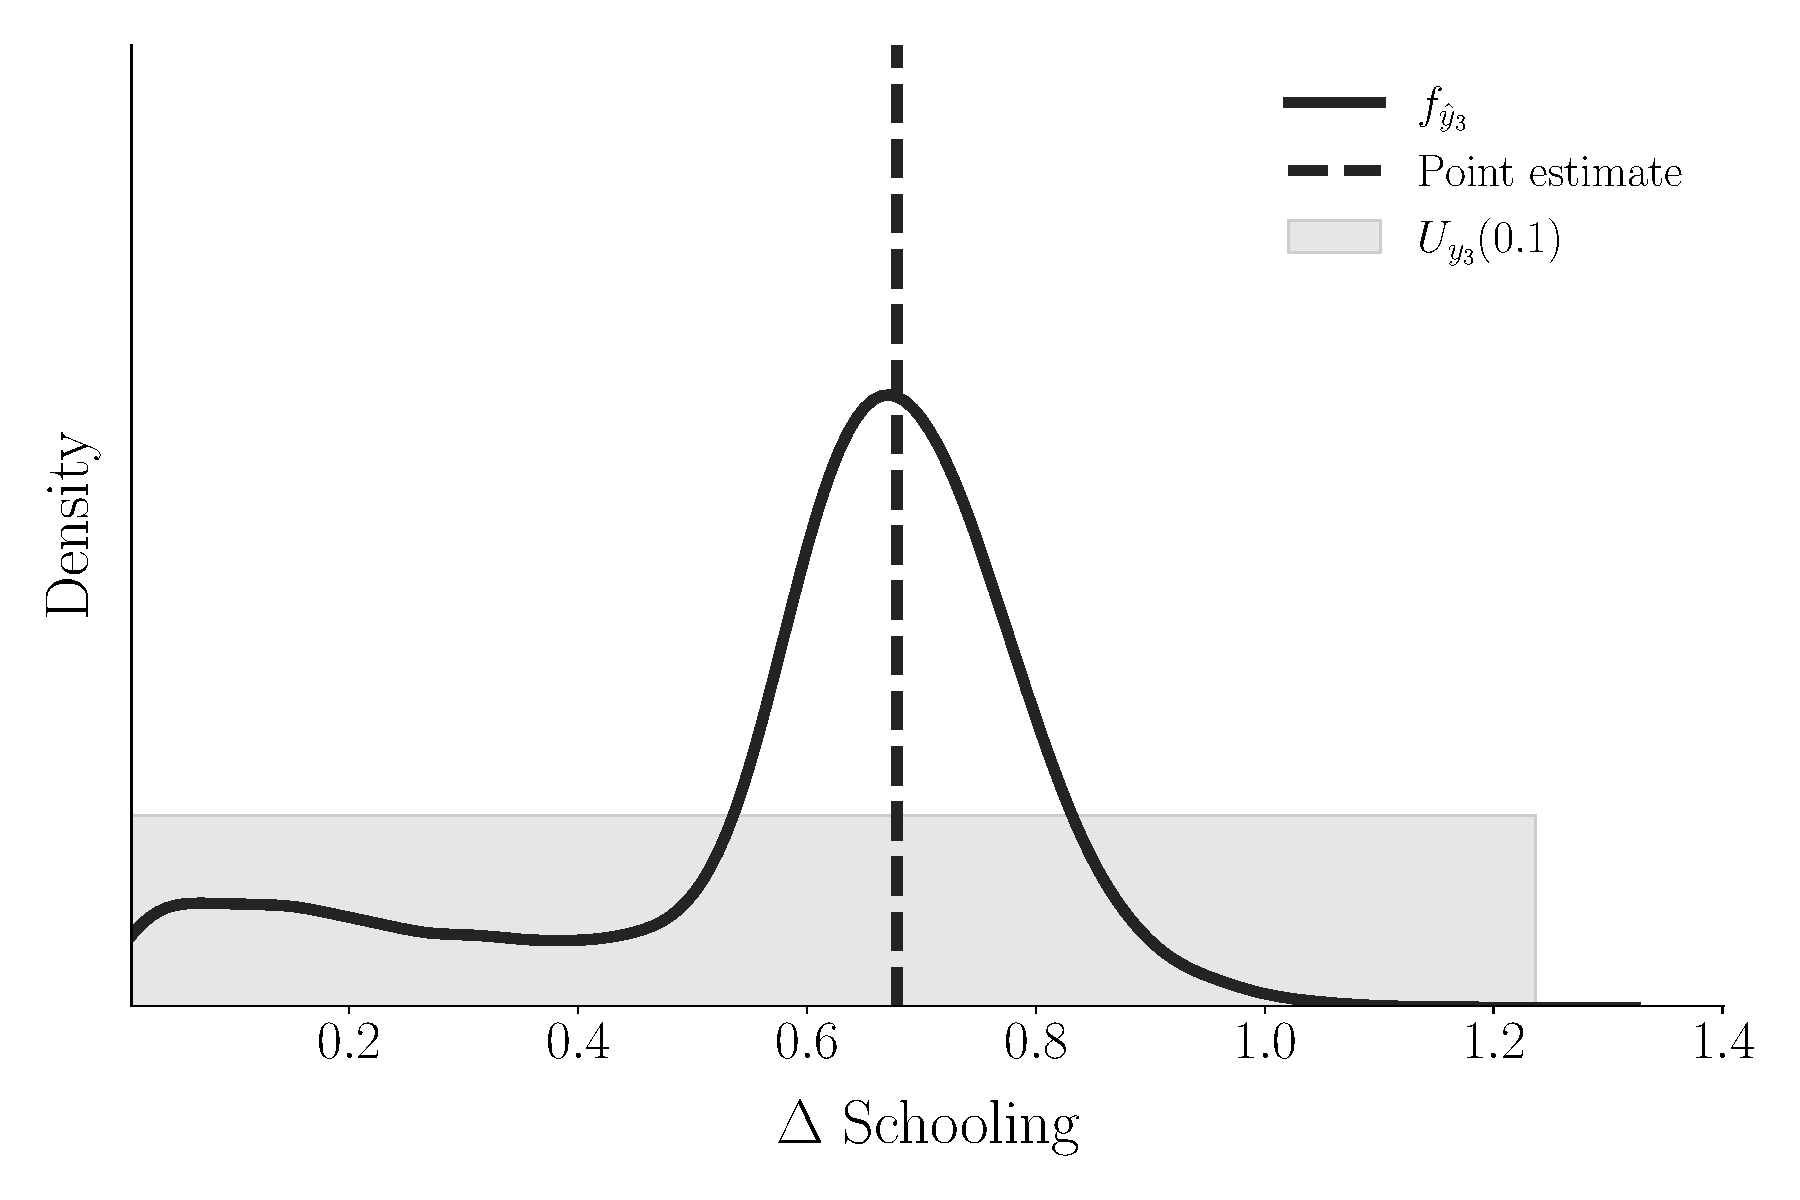
\includegraphics{fig-policy-average-years-type-2-bw}}}
  \subfloat[Type 4]{\scalebox{0.25}{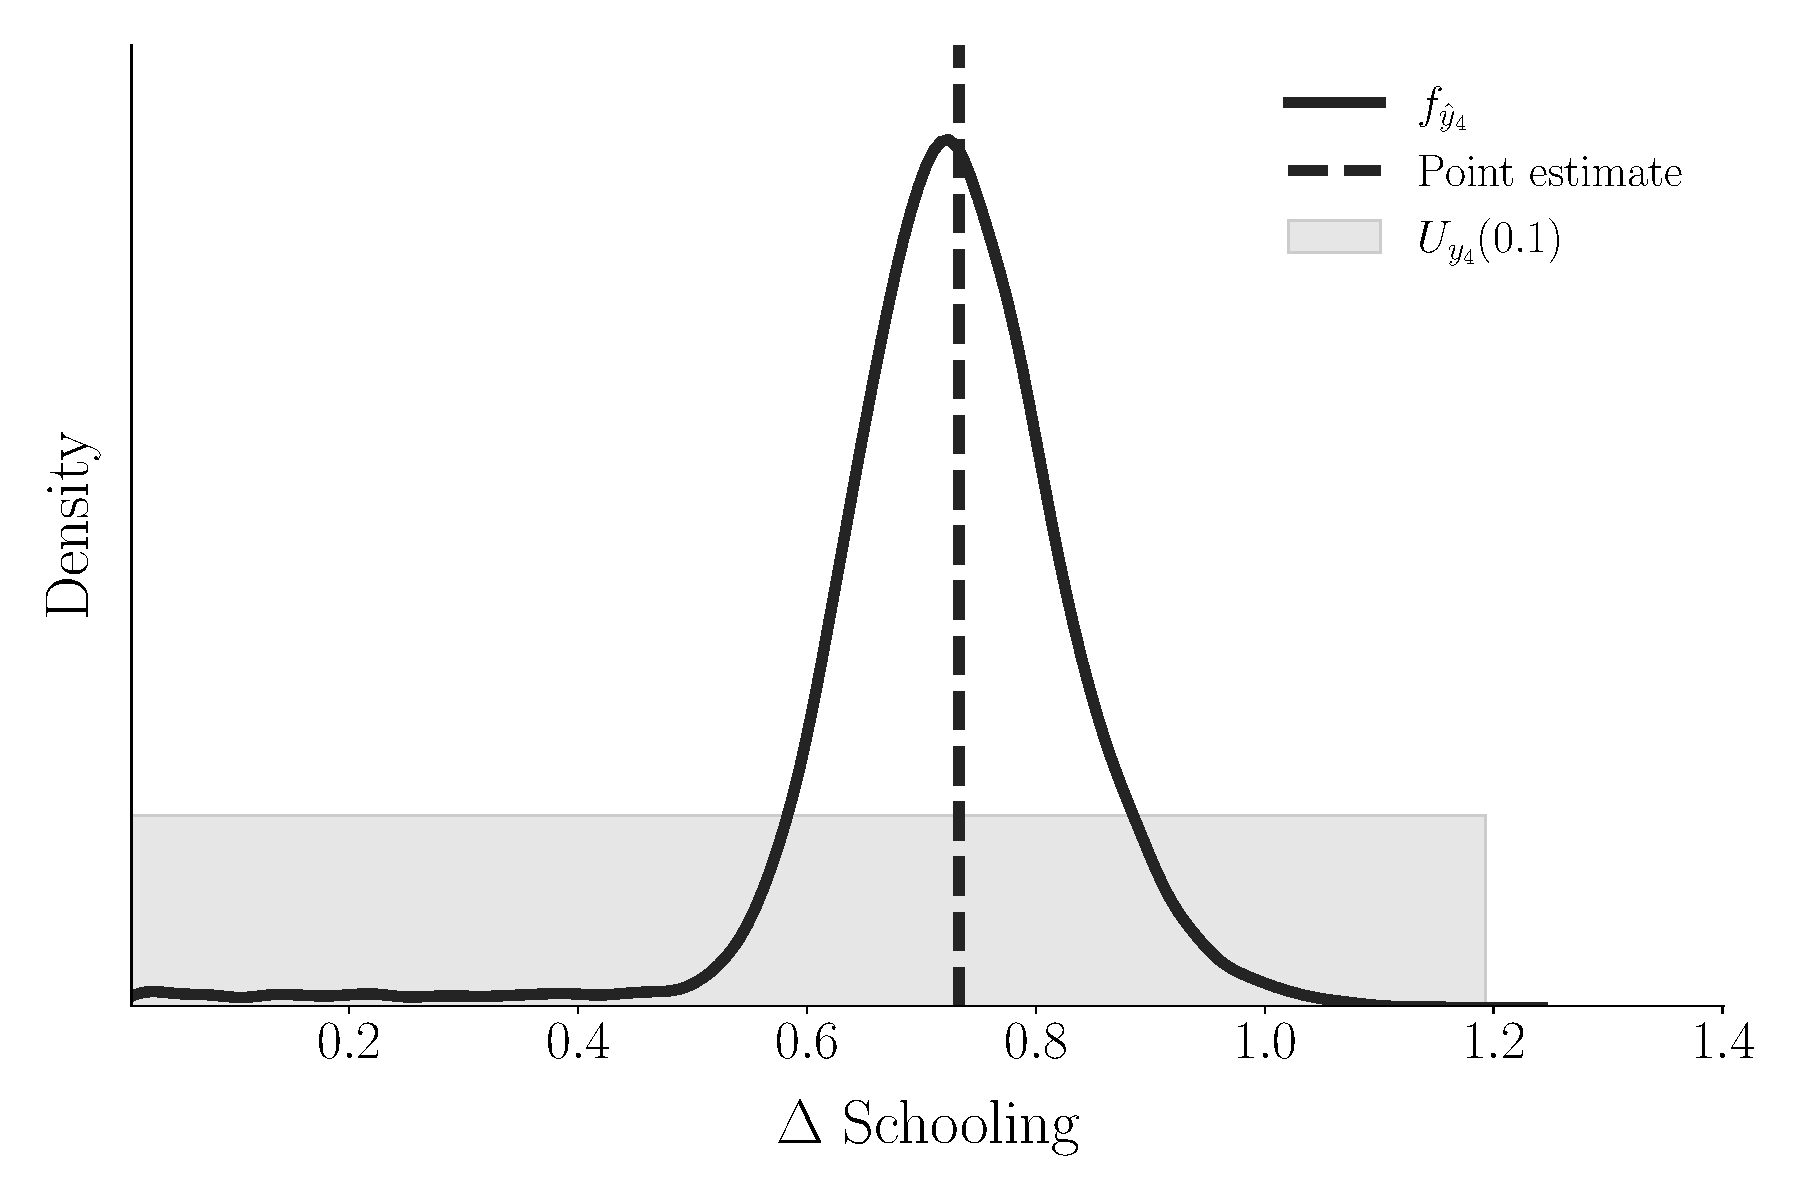
\includegraphics{fig-policy-average-years-type-3-bw}}}
  \caption{Targeted subsidy for all types}\label{Targeted subsidy for all types}
\end{figure}\FloatBarrier

\noindent Figure \ref{Policy impact and time preference} shows the impact of the tuition subsidy at the upper $\delta_H$ and lower $\delta_L$ bound of the estimated confidence set for $\delta$. The results for both scenarios are based on simulated samples of $10,000$ individuals.

\begin{figure}[h!]\centering
\subfloat[Low $\delta$]{\scalebox{0.25}{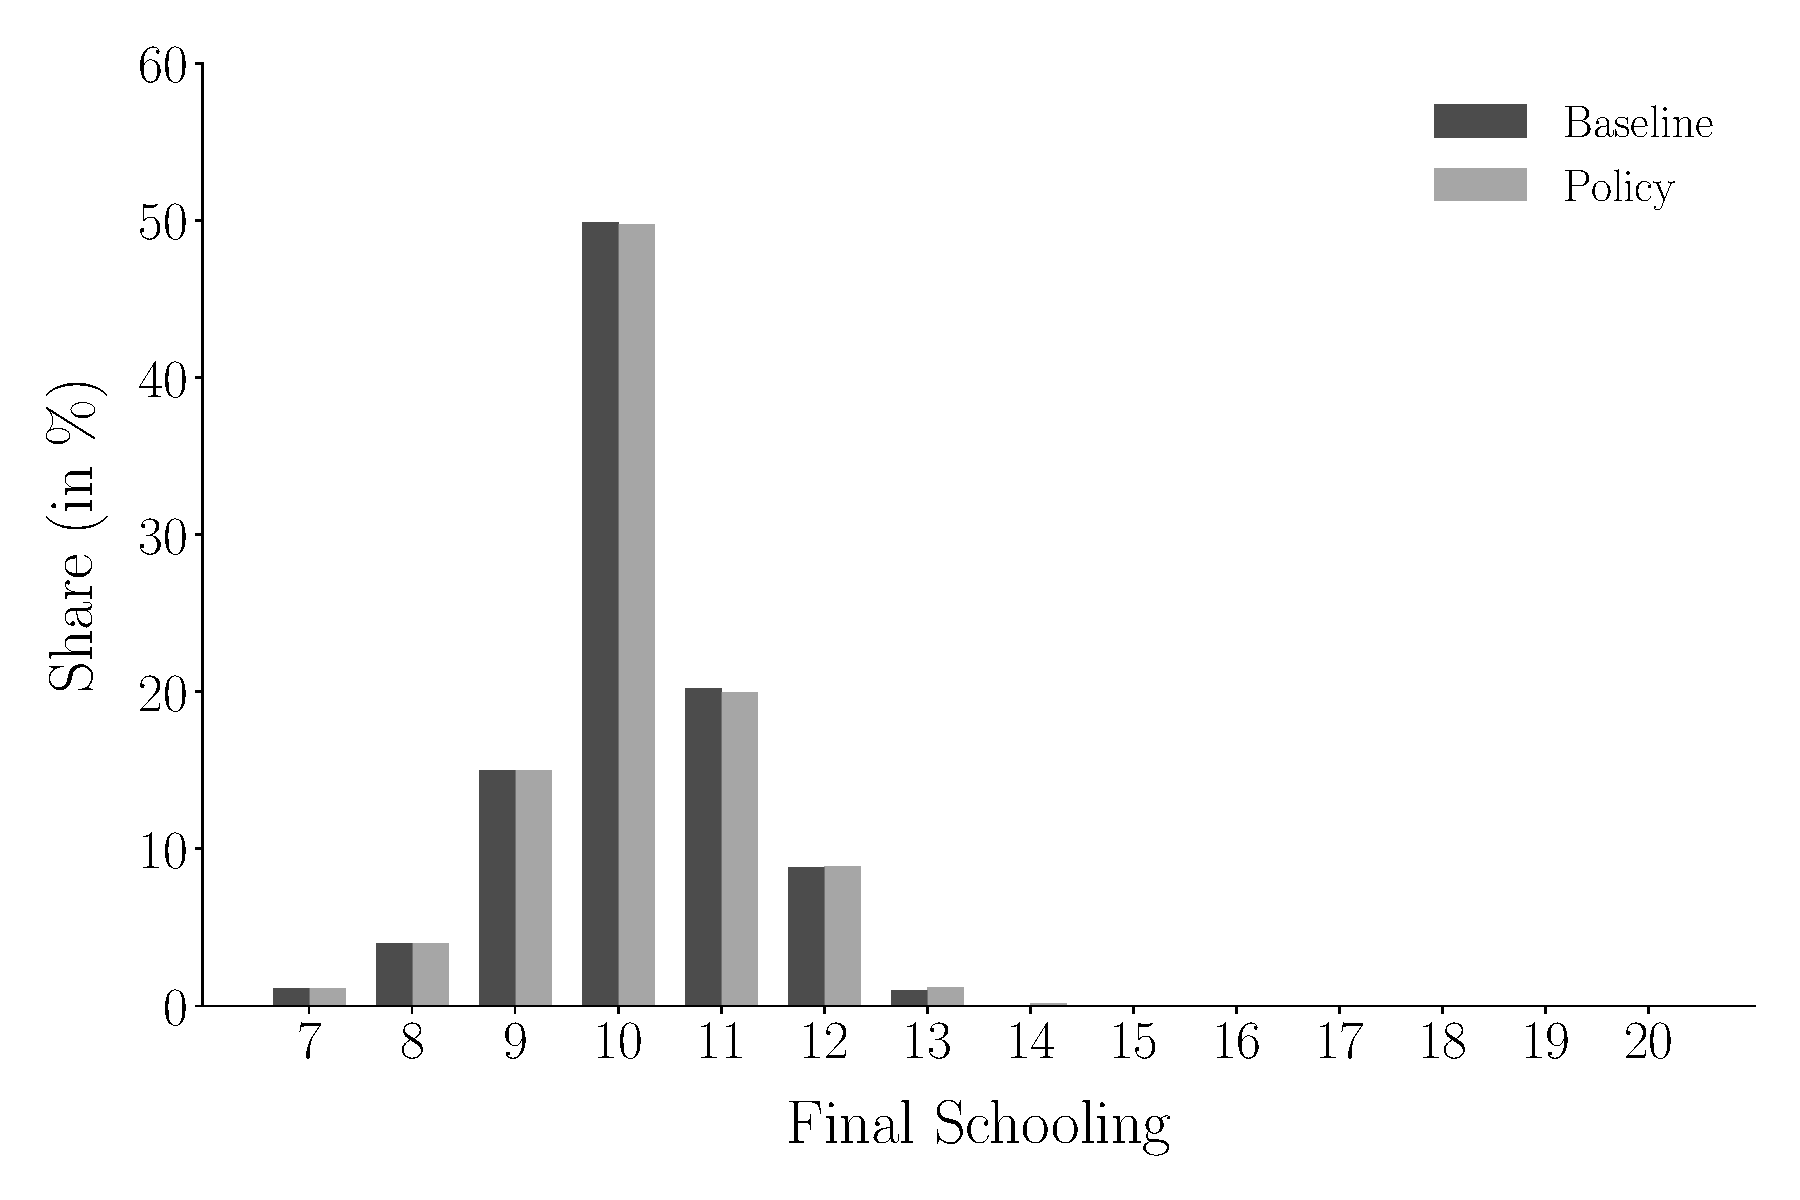
\includegraphics{fig-policy-impact-delta-low-bw}}\label{type 0}}
\subfloat[High $\delta$]{\scalebox{0.25}{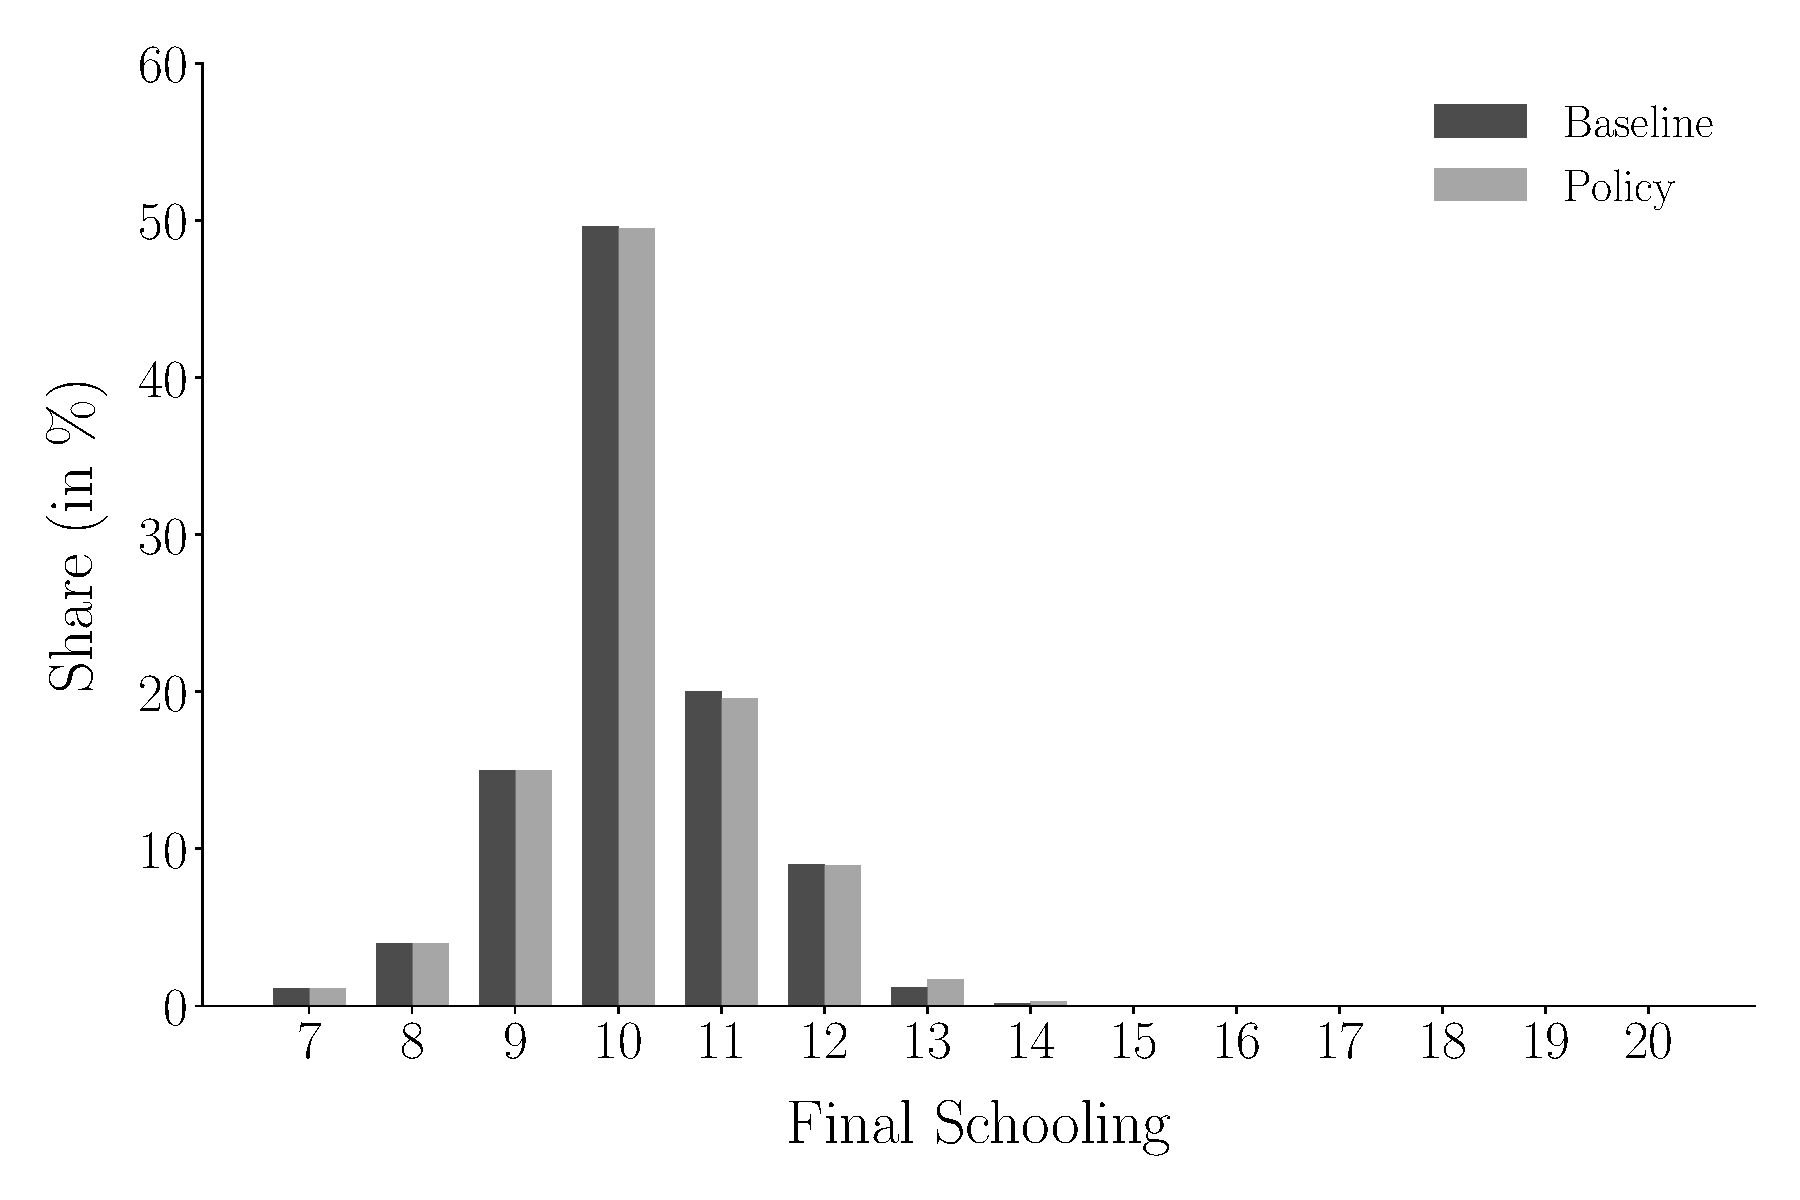
\includegraphics{fig-policy-impact-delta-high-bw}}\label{type 2}}
\caption{Policy impact and time preference}\label{Policy impact and time preference}
\end{figure}\FloatBarrier
